\documentclass[11pt,a4paper]{article}
\usepackage[utf8]{inputenc}
\usepackage[T1]{fontenc}
\usepackage{amsthm} %numéroter les questions
\usepackage[frenchb]{babel}
\usepackage{datetime}
\usepackage{xspace} % typographie IN
\usepackage{hyperref}% hyperliens
\usepackage[all]{hypcap} %lien pointe en haut des figures
\usepackage[french]{varioref} %voir x p y
\usepackage{fancyhdr}% en têtes
%\input cyracc.def
\usepackage[]{graphicx} %include pictures
\usepackage{pgfplots}
\usepackage[]{circuitikz}
\usepackage{ifthen}

\usepackage[top=1.3 in, bottom=1.3 in, left=1.3 in, right=1.3 in]{geometry} % Yeah, that's bad to play with margins
\usepackage[]{pdfpages}

\usepackage[]{attachfile}

\usepackage{float}
\usepackage{subfig}

\usepackage{todonotes} % \missingfigure
\usepackage{gensymb} % \ohm

\usepackage{framed}

\newdateformat{mydate}{2016--2017}%hack pour remplacer \THEYEAR


\newboolean{corrige}
\ifx\correction\undefined
\setboolean{corrige}{false}% pas de corrigé
\else
\setboolean{corrige}{true}%corrigé
\fi

%\setboolean{corrige}{false}% pas de corrigé

\newboolean{annexes}
\setboolean{annexes}{true}%annexes
%\setboolean{annexes}{false}% pas de annexes

\definecolor{darkblue}{rgb}{0,0,0.5}

\newboolean{mos}
%\setboolean{mos}{true}%annexes
\setboolean{mos}{false}% pas de annexes

\usepackage{aeguill} %guillemets

%% fancy header & foot
\pagestyle{fancy}
%Numero du TP :
\def \labonumber {Projet -- Cahier des charges }
\lhead{[ELEC-H-310] Choucroute numérique\\ \labonumber}
\rhead{\mydate\today\\ page \thepage}
\chead{\ifthenelse{\boolean{corrige}}{Corrigé}{}}
\cfoot{}
%%

\pdfinfo{
/Author (Quentin Delhaye, Ken Hasselmann, ULB -- BEAMS)
/Title (\labonumber ELEC-H-310)
/ModDate (D:\pdfdate)
}

\hypersetup{
pdftitle={\labonumber [ELEC-H-310] Choucroute numérique},
pdfauthor={Quentin Delhaye, Ken Hasselmann, ULB -- BEAMS},
pdfsubject={}
}

\theoremstyle{definition}% questions pas en italique
\newtheorem{Q}{Question}[] % numéroter les questions [section] ou non []

\newcommand{\reponse}[1]{% pour intégrer une réponse : \reponse{texte} : sera inclus si \boolean{corrige}
	\ifthenelse {\boolean{corrige}} {\paragraph{Réponse :} \color{darkblue}   #1\color{black}} {}
 }

\newcommand{\addcontentslinenono}[4]{\addtocontents{#1}{\protect\contentsline{#2}{#3}{#4}{}}}

\date{\vspace{-1.7cm}\mydate\today}
\title{\vspace{-2cm} \labonumber\\ Électronique numérique [ELEC-H-310]\\Conception d'une régulation de refroidissement\ifthenelse{\boolean{corrige}}{~\\Corrigé}{}}

%\author{\vspace{-1cm}}%\textsc{Yannick Allard}}

\setlength{\parskip}{0.2cm plus2mm minus1mm} %espacement entre §
\setlength{\parindent}{0pt}






%%%%%%%%%%%%%%%%%%%%%%%%%%%%%%%%%%%%%%%%%%%%%%%%%%%%%%%%%%%%%%%%%%%%%%%%%%%%%%%%%%%%%%%%%%%%%%%%%%%%%%%%%%%%%
%%%%%%%%%%%%%%%%%%%%%%%%%%%%%%%%%%%%%%%%%%%%%%%%%%%%%%%%%%%%%%%%%%%%%%%%%%%%%%%%%%%%%%%%%%%%%%%%%%%%%%%%%%%%%
%%%%%%%%%%%%%%%%%%%%%%%%%%%%%%%%%%%%%%%%%%%%%%%%%%%%%%%%%%%%%%%%%%%%%%%%%%%%%%%%%%%%%%%%%%%%%%%%%%%%%%%%%%%%%
% http://tex.stackexchange.com/questions/128123/circuitikz-current-source
% preparation to create bipoles

\makeatletter
\def\TikzBipolePath#1#2{\pgf@circ@bipole@path{#1}{#2}}

\pgf@circ@Rlen = \pgfkeysvalueof{/tikz/circuitikz/bipoles/length}
\makeatother

\newlength{\ResUp} \newlength{\ResDown}
\newlength{\ResLeft} \newlength{\ResRight}

% set default dohicky size

\ctikzset{bipoles/doohicky/height/.initial=.4}
\ctikzset{bipoles/doohicky/width/.initial=.6}

% create doohicky shape

\pgfcircdeclarebipole{}
 {\ctikzvalof{bipoles/doohicky/height}}
 {doohicky}
 {\ctikzvalof{bipoles/doohicky/height}}
 {\ctikzvalof{bipoles/doohicky/width}}
 {
    \pgfsetlinewidth{\pgfkeysvalueof{/tikz/circuitikz/bipoles/thickness}\pgfstartlinewidth}
    \pgfextractx{\ResRight}{\northeast}
    \pgfextracty{\ResUp}{\northeast}
    \pgfextractx{\ResLeft}{\southwest}

  \pgfmoveto{\pgfpoint{\ResLeft}{0cm}}
    \pgfpathellipse{\pgfpoint{0.333\ResLeft}{0cm}}{\pgfpoint{0.667\ResRight}{0cm}}{\pgfpoint{0cm}{\ResUp}}
  \pgfmoveto{\pgfpoint{\ResRight}{0cm}}
    \pgfpathellipse{\pgfpoint{0.333\ResRight}{0cm}}{\pgfpoint{0.667\ResRight}{0cm}}{\pgfpoint{0cm}{\ResUp}}
  \pgfusepath{draw} %draw doohicky
    \pgfscope
    \pgfsetarrowsend{latex'}
    \pgfpathmoveto{\pgfpoint{0.667\ResLeft}{1.333\ResUp}}
    \pgfpathlineto{\pgfpoint{0.667\ResRight}{1.333\ResUp}}
    \pgfusepath{draw}   %draw arrow
    \endpgfscope
 }

% create doohicky to-path style

\def\doohickypath#1{\TikzBipolePath{doohicky}{#1}}
\tikzset{doohicky/.style = {\circuitikzbasekey, /tikz/to path=\doohickypath, l=#1}}

% end of setup
%%%%%%%%%%%%%%%%%%%%%%%%%%%%%%%%%%%%%%%%%%%%%%%%%%%%%%%%%%%%%%%%%%%%%%%%%%%%%%%%%%%%%%%%%%%%%%%%%%%%%%%%%%%%
%%%%%%%%%%%%%%%%%%%%%%%%%%%%%%%%%%%%%%%%%%%%%%%%%%%%%%%%%%%%%%%%%%%%%%%%%%%%%%%%%%%%%%%%%%%%%%%%%%%%%%%%%%%%
%%%%%%%%%%%%%%%%%%%%%%%%%%%%%%%%%%%%%%%%%%%%%%%%%%%%%%%%%%%%%%%%%%%%%%%%%%%%%%%%%%%%%%%%%%%%%%%%%%%%%%%%%%%%





















\begin{document}
\pagestyle{empty}
\maketitle
% \vspace*{-1cm}


% ########   ##      ##  ##########  ########     #####
%    ##      ###     ##      ##      ##     ##  ##     ##
%    ##      ## ##   ##      ##      ##     ##  ##     ##
%    ##      ##  ##  ##      ##      ########   ##     ##
%    ##      ##   ## ##      ##      ##   ##    ##     ##
%    ##      ##     ###      ##      ##    ##   ##     ##
% ########   ##      ##      ##      ##     ##    #####

\section{Introduction}
Le but de ce projet est de réaliser un système de contrôle de la température analogue à celui que l'on trouve dans les ordinateurs portables.
Grâce au courant d'air généré par un ventilateur à vitesse variable, on maintient la température du redroidisseur du processeur dans les limites imposées et ce, malgré des variations dans la puissance du processeur liées à sa charge de calcul.

\begin{center}
\begin{figure}[H]
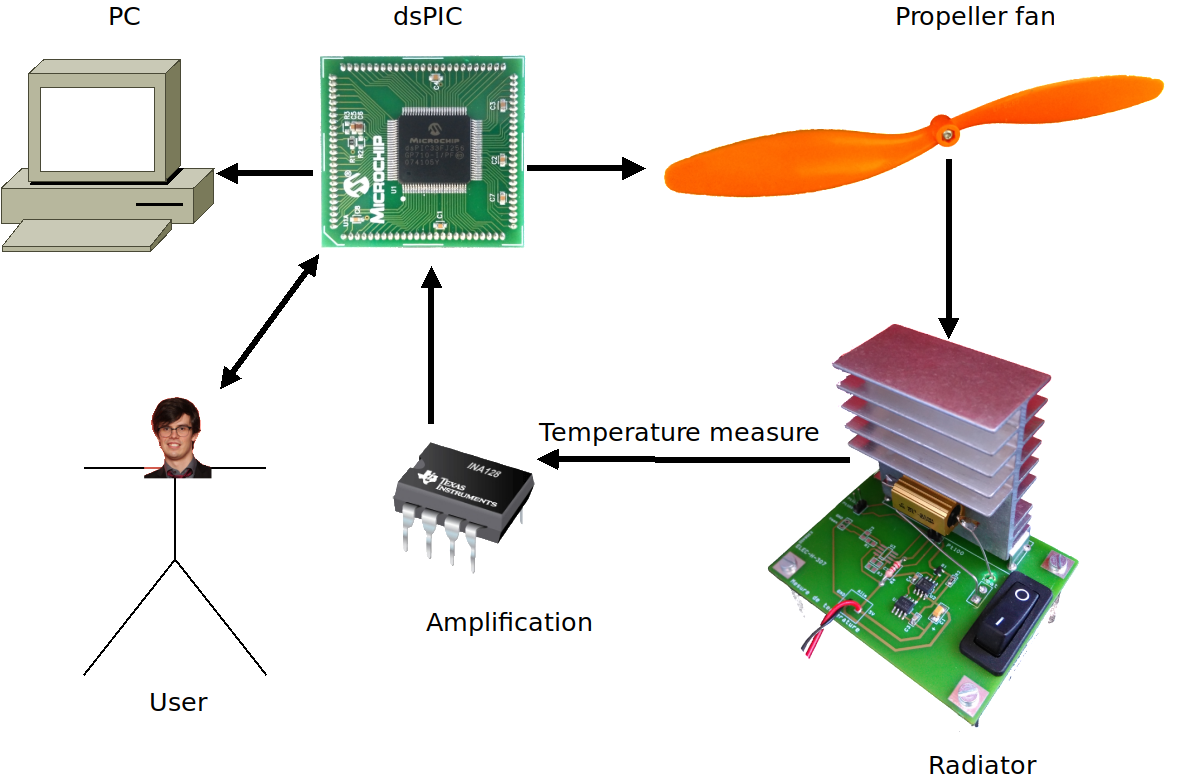
\includegraphics[width=\textwidth]{workflow}
\caption{Diagramme du projet}
\label{fig:workflow}
\end{figure}
\end{center}

Dans ce projet, vous disposerez de~:
\begin{itemize}
	\item La carte à microcontrôleur dsPIC du labo.
	\item Une hélice entraînée par;
	\item Un moteur à courant continu qui joue le rôle de ventilateur.
	\item Une sonde de température
	\item Une résistance chauffante montée sur un refroidisseur incarnant le processeur qui dissipe de la puissance.
	\item Un clavier.
	\item Un écran LCD.
	\item Une connexion série avec un ordinateur permettant permettant d'afficher l'évolution de la température dans le temps.
\end{itemize}




%  #######      ###     ##     ##  ########   #########  ########
% ##     ##    ## ##    ##     ##     ##      ##         ##     ##
% ##          ##   ##   ##     ##     ##      ##         ##     ##
% ##         ##     ##  #########     ##      ######     ########
% ##         #########  ##     ##     ##      ##         ##   ##
% ##     ##  ##     ##  ##     ##     ##      ##         ##    ##
%  #######   ##     ##  ##     ##  ########   #########  ##     ##



\section{Cahier des charges}
Le projet étant relativement complexe, nous allons décrire les différentes demandes.

Afin de contrôler la température de la pièce chauffante, vous serez amenés à faire tourner une hélice
à vitesse variable.
Pour ce faire, vous devrez faire varier la tension d’alimentation délivrée au moteur de l’hélice.

Comme lors des laboratoires d’électronique appliquée, ce moteur est alimenté par un amplificateur de puissance commandé par une onde carrée de type PWM (voir section~\ref{sec:helice}).
Il sera dès lors nécessaire de concevoir un système capable de générer des ondes carrées réglables à volonté.
La période de l’onde carrée devra être courte par rapport à la constante mécanique du moteur (la vitesse du moteur doit être pratiquement constante lors d’une période de la PWM).

En mesurant la température de la résistance chauffante, vous pourrez ajuster la vitesse du moteur en réalisant une boucle de régulation numérique au sein de votre programme.
Cette régulation pourra ici être très simple (un simple régulateur proportionnel), mais rien ne vous empêche de concevoir une boucle plus complexe si vous le désirez.

\begin{center}
\framebox{En régime, l’erreur sur la température devra être inférieure à un degré Celsius}
\end{center}

La mesure de température est réalisée au moyen d’une résistance de platine du type Pt100.
La résistance de ce composant varie linéairement avec la température selon la loi $R(T) = 100\ohm + \alpha T$, où $\alpha = 0.385\ohm/\celsius$ et $T$ est la température exprimée en degrés Celsius.
En faisant passer un courant constant à travers la résistance, nous obtenons une différence de potentiel variable avec la température.
À l’aide d’un amplificateur différentiel, vous serez amenés à conditionner cette tension avant de pouvoir la numériser.
Le circuit de mesure complet est décrit plus loin.

\begin{center}
\framebox{Nous supposons que la température ne dépasera pas $45\celsius$}
\end{center}

Un utilisateur devra pouvoir interagir avec le comportement de l'ensemble à travers le couple clavier + écran LCD présents sur la carte de développement.
Votre fonction de gestion du clavier permettra de transformer une séquence de touches en commandes pour votre système~:
\begin{itemize}
	\item Touche 'A' + deux chiffres~: changement de la température de commande.
	Exemple~: «~A23~» pour fixer la temérature voulue à $23\celsius$.
	\item Touche 'B' + autre chiffres~: changement de la période d'échantillonnage, en millisecondes.
	Exemple~: «~B0250~» pour fixer la période à $250\ ms$.
	Votre système devra accepter des périodes allant de $1\ ms$ à $1\ s$.
	\item La touche 'F' sert à entrer définitivement la commande.
	Avant d'appuyer sur cette touche, la séquence entrée doit être affichée sur l'écran LCD.
	\item La touche 'C' permet de supprimer le dernier caractère entré.
	\item La touche 'D' annule la saisie de caractères.
\end{itemize}

En temps normal, la température sera affichée sur l’écran LCD et sera rafraîchie toutes les secondes.
Le format d’affichage est le suivant : «~23.4C~»

Il s'agira ensuite pour finir d'ajouter l'envoi des données sur le pc via le port
serie. On utilisera pour ça le périphérique UART du dsPIC.
Il données devront être envoyés toutes les secondes sous cette forme : «~25.3\textbackslash n~».

On utilisera ensuite le script python \textit{graph.py} sur les ordinateurs pour visualiser
les données.

\begin{figure}[H]
\center
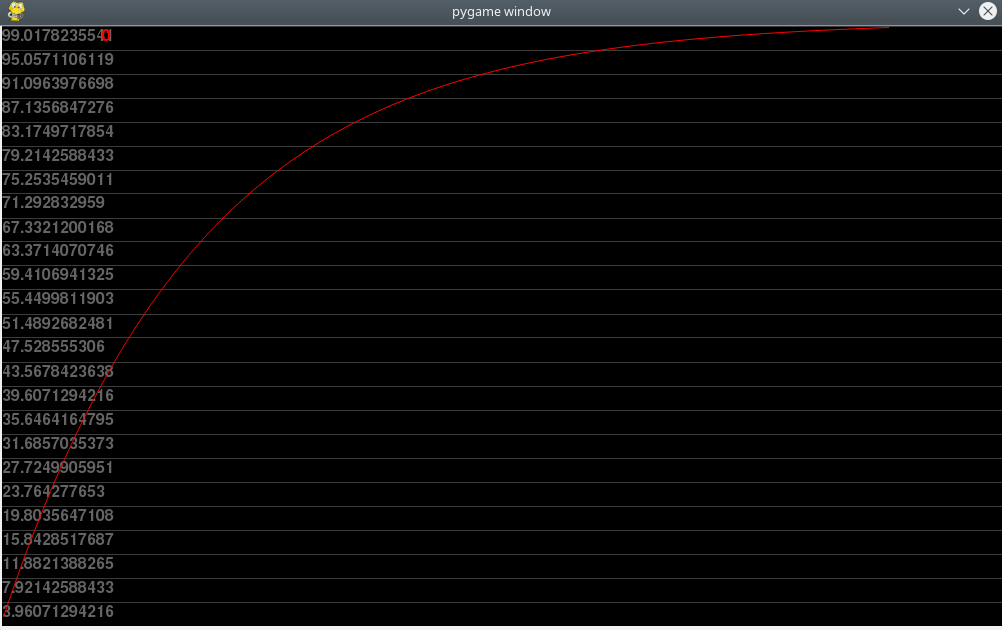
\includegraphics[width=0.7\textwidth]{graph}
\caption{Visuel du script d'affichage des données sur le PC.}
\label{fig:graphpy}
\end{figure}

%\todo[inline]{Présentation du script de Ken}




% ########   #########  #########  ##         #########  ##    ##   ########     #####    ##      ##
% ##     ##  ##         ##         ##         ##          ##  ##       ##      ##     ##  ###     ##
% ##     ##  ##         ##         ##         ##           ####        ##      ##     ##  ## ##   ##
% ########   ######     ######     ##         ######        ##         ##      ##     ##  ##  ##  ##
% ##   ##    ##         ##         ##         ##           ####        ##      ##     ##  ##   ## ##
% ##    ##   ##         ##         ##         ##          ##  ##       ##      ##     ##  ##     ###
% ##     ##  #########  ##         #########  #########  ##    ##   ########     #####    ##      ##


\section{Mode opératoire}
Avant d’entamer un projet de cette envergure, il vous sera nécessaire de bien réfléchir à l’ordre de vos actions.

Il est fortement conseillé de commencer par réinterpréter le cahier des charges sous forme de schéma bloc fonctionnel comprenant les fonctions de base du projet.
Par chacune de ces fonctionnalités, isolez les périphériques à utiliser et réalisez un schéma de principe de votre algorithme.

Une fois ce travail préparatoire terminé, attaquez le projet bloc par bloc.
Commencez par une fonctionnalité simple comme la commande en vitesse de l’hélice et ajoutez ensuite le reste du projet petit à petit.

Ne réalisez pas de programme trop spécifique à une fonctionnalité~: rappelez-vous que les différentes parties de votre algorithme devront dialoguer entre elles.
À ce titre, il est avantageux de directement réaliser les interfaces des blocs à réaliser.
Par exemple, pensez à prévoir une fonction permettant de modifier simplement la vitesse de l’hélice, car vous en aurez besoin plus tard.

L’objectif premier du projet est que vous arriviez à programmer un système tout en comprenant bien le programme que vous réalisez~: inutile d’aller trop vite~!





% ##       ##  #########   #######   ##     ##  ########   #########
% ###     ###  ##         ##     ##  ##     ##  ##     ##  ##
% ## ## ## ##  ##         ##         ##     ##  ##     ##  ##
% ##  ###  ##  ######      #######   ##     ##  ########   ######
% ##       ##  ##                ##  ##     ##  ##   ##    ##
% ##       ##  ##         ##     ##  ##     ##  ##    ##   ##
% ##       ##  #########   #######    #######   ##     ##  #########


\section{Mesure de la température}
Comme dit précédemment, la mesure de température est réalisée au moyen d’une résistance de platine traversée par un courant continu de $1 mA$.
Le schéma électronique est donné sur la figure~\ref{fig:mes-temp}.

\begin{figure}[H]
\shorthandoff{:!;}
\center
	\subfloat[\label{fig:mes-temp-ampop}]{%
		\parbox[b]{.45\linewidth}{% Embed the content of the subfloat into a parbox to make it wider. Otherwise, the width of the subfloat is set by the width of the table, and so is the caption.
		\center
			\begin{circuitikz}
				\draw
				(0,0) node[op amp] (opamp) {}
				(3,0) node[npn] (npn) {}
				(opamp.out) --(npn.base)
				(npn.collector) to[vR=Pt100] +(0,2) to [short, -o] +(1,0) node (A) {}
				($(npn.collector)+(0,2.5)$) node (vdd) {5V}

				(npn.collector) to [short, -o] +(1,0) node (B) {}
				(A) to[open, v^=$V_{mes}$] (B)

				(npn.emitter) to[short] +(0,-0.5) node(C) {}
				(C) to[R=$R_1$] +(0,-2) node [ground] {}
				($(C)+(0.01,0)$) -| (opamp.+)% For some reason, putting "(C) -| (opamp.+)" leaves a horizontal gap between C and the wire.
				;
			\end{circuitikz}
		}
	}
	\subfloat[\label{fig:mes-temp-current-source}]{%
		\parbox[b]{.45\linewidth}{%The [b] sets the content to be positioned at the bottom of the box.
		\center
			\begin{circuitikz}
				\draw
				(0,-2) to [vR=Pt100] (0,0)
				(0,-2) to [doohicky, l=$1\ mA$] +(0,-2) node [ground] {}
				(0,0.5) node (vdd) {5V}
				(0,0) to [short, -o] (1,0) node (A) {}
				(0,-2) to [short, -o] (1,-2) node (B) {}
				(A) to[open, v^=$V_{mes}$] (B)
				;
			\end{circuitikz}
		}
	}
\caption{Mesure de la température à l'aide d'une résistance Pt100.}
\label{fig:mes-temp}
\shorthandon{:!;}
\end{figure}

L’ensemble ampli-op + transistor (figure~\ref{fig:mes-temp-ampop}) peut être vu comme une source de courant contrôlable (figure~\ref{fig:mes-temp-current-source})~: en imposant la tension sur la résistance $R_1$ par le zéro virtuel de l’ampli-op, nous fixons en même temps le courant à travers le transistor.
Ce courant circule ensuite dans la sonde Pt100, ce qui provoque l’apparition à ses bornes d’une tension variant linéairement avec la température.

Cette mesure présente deux défauts~: non seulement elle n’est pas référencée à la masse, mais en plus elle est de faible amplitude.
Nous allons dès lors utiliser un amplificateur différentiel chargé d’amplifier la différence de potentiel aux bornes de la résistance, tout en atténuant fortement la tension de mode commun d'environ 5~V.

À l’aide d’un amplificateur INA128 dont la notice se trouve en annexe, vous devrez réaliser sur protoboard le montage permettant de récupérer la tension et de l’adapter aux niveaux d’entrée du convertisseur analogique-numérique du dsPIC (0~V -- 3.3~V).





% ##     ##  #########  ##         ########    #######   #########
% ##     ##  ##         ##            ##      ##     ##  ##
% ##     ##  ##         ##            ##      ##         ##
% #########  ######     ##            ##      ##         ######
% ##     ##  ##         ##            ##      ##         ##
% ##     ##  ##         ##            ##      ##     ##  ##
% ##     ##  #########  #########  ########    #######   #########


\section{Circuit d'alimentation de l'hélice}\label{sec:helice}
Le dsPIC n’est pas suffisamment puissant pour alimenter un moteur.
Comme c’était le cas pour l’amplificateur audio, nous devons ajouter un circuit d’amplification de puissance (une extension de la catégorie \textit{buffers} utilisée dans un laboratoire précédent).
Cette fois, nous allons utiliser un amplificateur à commutation, ce qui signifie qu’il fournit à sa sortie une onde carrée et non un signal continu.
Son schéma de principe est tracé sur la figure~\ref{fig:alim-moteur}.

% \missingfigure[figwidth=\textwidth]{Alimentation moteur}
\begin{figure}[H]
\center
\shorthandoff{:!;}
\begin{circuitikz}
	\draw
	(1,0) node [nmos] (nmos1) {}%anchors are drain, source and gate.
	(1,1.5) node [pmos] (pmos1) {}% 1 = bottom pair
	(1,5) node [nmos] (nmos2) {}% 2 = top pair
	(1,6.5) node [pmos] (pmos2) {}
	(pmos2.source) node[above] () {5V}%Between parenthesis should be the label of the node. Don't any, here.
	(nmos2.source) node [ground] () {}
	(pmos1.source) node[above] () {5V}
	(nmos1.source) node[ground] () {}

	($(nmos2.drain)-(2,0)$) node [left]() {IN1} to [short, -*] +(1,0) node (A) {} -| (pmos2.gate)
	(A) -| (nmos2.gate)

	($(nmos1.drain)-(2,0)$) node [left]() {IN2} to [short, -*] +(1,0) node (B) {} -| (pmos1.gate)
	(B) -| (nmos1.gate)

	(pmos2.drain) to [short] +(3,0) to [twoport,t={Moteur}, bipoles/twoport/height=1.5] +(0,-4) |- (pmos1.drain)
	;
\end{circuitikz}
\shorthandon{:!;}
\caption{Alimentation du moteur.}
\label{fig:alim-moteur}
\end{figure}

Chaque branche du convertisseur peut être vue comme un inverseur à MOS~: lorsque la commande d’une branche est à l’état haut, le transistor du bas est rendu passant alors celui du haut de la branche est coupé.
La différence par rapport aux circuits logiques classiques est que les transistors sont ici capables de fournir des courants nettement plus élevés.

L’avantage de ce système par rapport à une amplification classique est qu’il possède un rendement élevé.
En première approximation, aucune puissance n’est dissipée dans les interrupteurs, ce qui implique que le rendement de l’alimentation est proche de 100~\%.
Une entrée supplémentaire, nommée \texttt{INHIB}, permet de désactiver l’alimentation en forçant 0~V sur les deux pattes de sortie quel que soit l’état des entrées.

La commande de l’amplificateur de puissance se fait à l’aide d’une onde carrée.
Diverses définitions sont associées à ce type de signal présenté à la figure~\ref{fig:square-wave}~:

% \missingfigure[figwidth=\textwidth]{Figure onde carée avec temps de montée et de descente.}
\begin{figure}[H]
\center
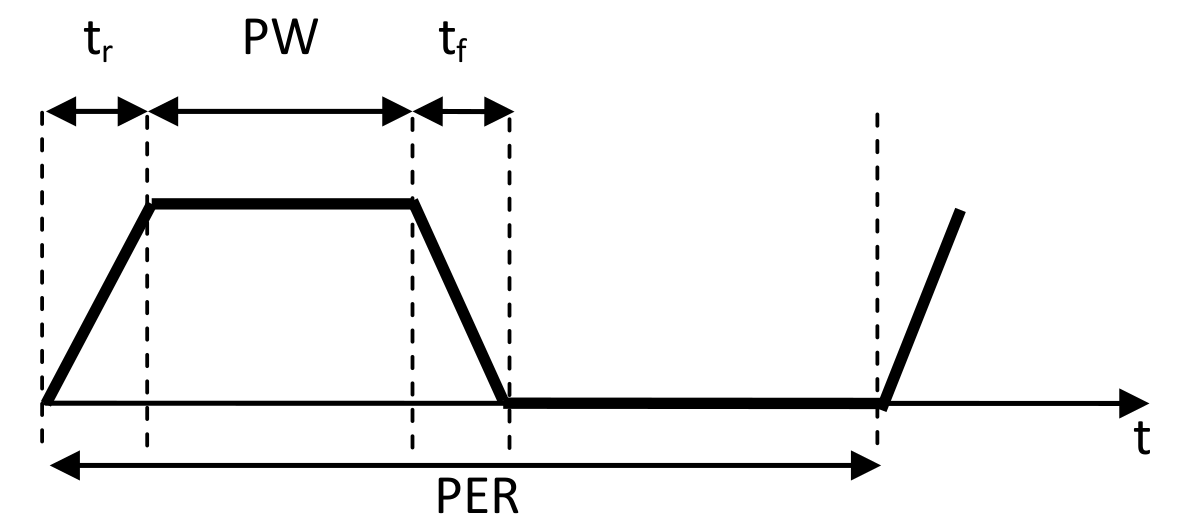
\includegraphics[width=0.6\textwidth]{square-wave}
\caption{Onde carrée.}
\label{fig:square-wave}
\end{figure}

Les différents temps caractéristiques sont les suivants~:
\begin{itemize}
	\item $PW$~: Pulse Width, la durée de l'état haut.
	\item $PER$~: la période du signal.
	\item $t_r$~: Rising time, le temps de montée.
	\item $t_f$~: Falling time, le temps de descente.
\end{itemize}

Dans la majorité des cas, y compris ici, les temps de montée et de descente sont négligeables.

Une autre caractéristique du signal est son rapport cyclique~: il est dfini comme \[D = \frac{PW}{PER}\]
et correspond à la proportion du temps pasée à l'état haut.

La commande PWM (\textit{Pulse Width Modulation}) consiste à un envoyer à un circuit de puissance une
onde carrée de période constante.
Il suffit dès lors de modifier le rapport cyclique pour moduler la valeur moyenne du signal.

Dans le cas de notre ampli de puissance, cela correspond à la tension moyenne imposée aux bornes
du moteur.
Prenons par exemple le signal de commande sortant du PIC à la figure~\ref{fig:pwm}~:

% \missingfigure[figwidth=\textwidth]{PWM}
\begin{figure}[H]
\center
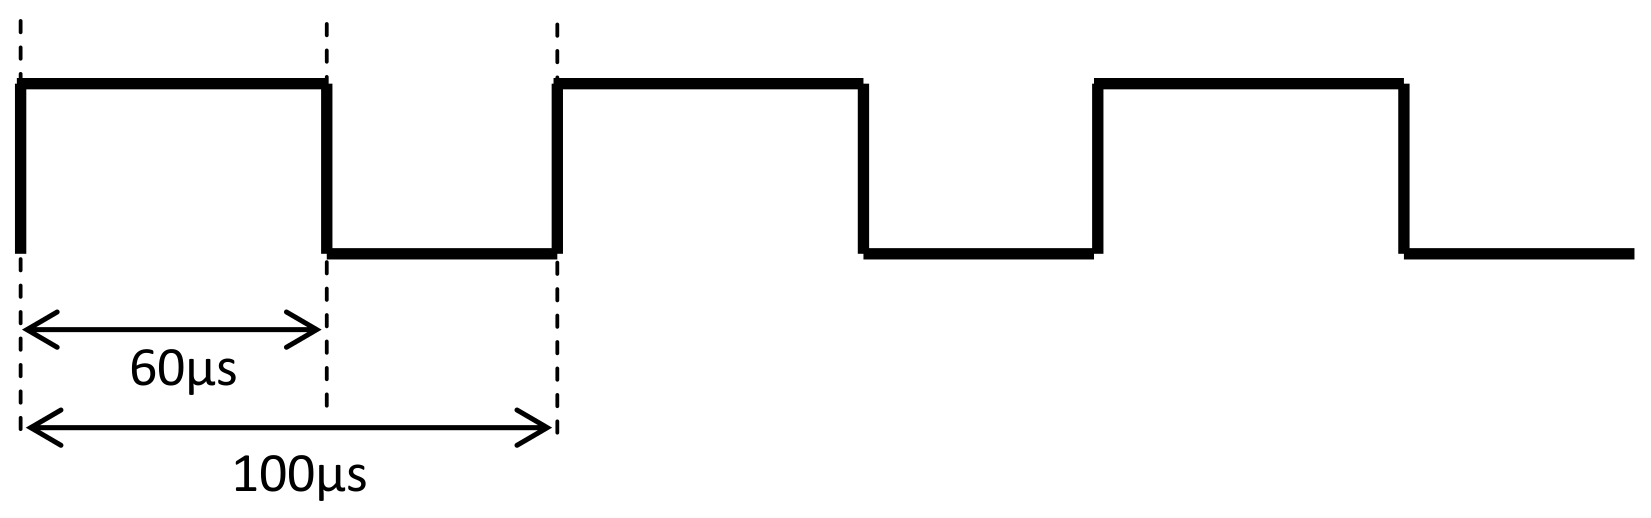
\includegraphics[width=0.7\textwidth]{pwm}
\caption{Signal PWM avec un rapport cyclique de 60~\%.}
\label{fig:pwm}
\end{figure}

Ce signal est imposé sur la borne \texttt{IN1} du moteur, \texttt{IN2} étant connectée la masse (V- est donc en
permanence connectée à la masse).

La période est de $100 \mu s$ et le rapport cyclique de 60~\%.
Lorsque la commande est à l’état haut, V- est connectée à la masse et le convertisseur impose 5~V aux bornes du moteur.
Dans le cas contraire, la différence de potentiel est de 0~V.
La tension moyenne est donc de $0.6 \cdot 5V  = 3 V$.

\begin{framed}
En jouant sur le rapport cyclique, vous pourrez faire varier la vitesse de l’hélice.\newline{}C'est donc cette
grandeur qui devra sortir de votre régulateur.
\end{framed}

Le dsPIC intègre un périphérique permettant de générer des ondes PWM~: il suffit de définir sa période et d’ensuite modifier un registre spécifique
pour modifier la durée de l’état haut.





\end{document}
